
\section{Rauschen}

Dieser Abschnitt soll einen groben Überblick über die verschiedenen Arten von Rauschen und ihre Ursachen liefern.

\subsection{Thermisches Rauschen}
Das thermische Rauschen wird von den statistischen Bewegungen der freien Ladungsträger, meist Elektronen, verursacht. Das thermische Rauschen ist weiterhin von der Frequenz unabhängig, weshalb es oft als weißes Rauschen bezeichnet wird.
Die Rauschspannung $u_R$, an einem Widerstand $R$, kann mit folgender Formel berechnet werden: 
\begin{align}
    u_R = \sqrt{4kTRB} \qquad \text{mit} \quad B = f_{max} - f_{min}
    \label{eq:thR}
\end{align}
Wobei T die absolute Temperatur ist und k die Boltzmannkonstante. B bezeichnet die Bandbreite des Messgerätes. Da es sich um statistische Schwankungen handelt, ergibt eine Mittelung von $u_R$ über die Zeit Null.\\
Aus obiger Formel \ref{eq:thR} kann durch die Division durch R eine Formel für die Rauschleistung hergeleitet werden.
\begin{align}
    P_R = 4kTB
\end{align}
Es geht klar hervor, dass die Rauschleistung nur von Temperatur und Frequenz abhängt. Somit wäre es also theoretisch möglich das thermische Rauschen, durch Kühlung des Versuchsaufbaus auf den absoluten Nullpunkt, abzustellen. Dies ist jedoch nicht praktikabel, da es mit enormen Kosten und Aufwand verbunden wäre \citep{VA}.

\subsection{Schrotrauschen}
Wie das thermische Rauschen ist auch das Schrotrauschen ein statisches und von der Frequenz unabhängiges Rauschen, weshalb es ebenfalls ein weißes Rauschen ist. Die Ursache ist jedoch die Quantelung der elektrischen Ladung, welche sich ebenfalls stochastisch bewegen und somit das Schrotrauschen verursachen. Der Effektivwert des Rauschstroms $i_R$ kann durch folgende Formel ausgedrückt werden:
\begin{align}
    i_R^2 = 2eIB
\end{align}
Wobei B wieder die Bandbreite des Messgerätes ist, e die Elektronenladung und I der fließende Gleichstrom.
Für die Rauschleistung $P_R$, über einen Übergang mit Widerstand $R$, gilt: 
\begin{align}
    P_R = i_R^2 R = 2eIRB
\end{align}
Aus dieser Formel ist ableitbar, dass das Schrotrauschen durch die Erniedrigung des Gleichstroms, der durch den Übergang fließt, erreicht werden kann \citep{VA}.

\subsection{Funkelrauschen}
Durch Störstellen im Material kann es zu Funkelrauschen kommen, welches mit zunehmender Frequenz abnimmt. Deshalb wird es auch als $\frac{1}{f}$ Rauschen bezeichnet. Abhilfe schafft hier, die Messungen bei hohen Frequenzen durchzuführen \citep{VA}.

\newpage
\section{Umwelteinflüsse}
\label{sec:umwelt}
Häufig ist bei Messungen jedoch nicht nur Rauschen ein Problem, sondern störende Umwelteinflüsse. Unsere Umwelt ist voll von Störquellen wie elektromagnetischen Wellen, beispielsweise von Radiosendern, welche die Messungen verfälschen, da Kabel im Versuchsaufbau für diese als Antenne fungieren können. Eines der stärksten Störeinflüsse ist wohl das Netzbrummen, was durch die öffentliche Stromversorgung bei 50 Hz verursacht wird. Ebenso können diverse elektrische Geräte wie Elektromotoren oder alte Röhrenmonitore Störungen verursachen \citep{VA}.\\

Um die Einstrahlung von störenden elektromagnetischen Wellen zu vermeiden ist eine gute Abschirmung von diesen vonnöten.
Darum werden die Messgeräte abgeschirmt und Koaxialkabel verwendet. Ein Koaxialkabel besteht aus einem Draht, welche von einer Isolierschicht umgeben ist, welche wiederum durch ein Drahtgeflecht umgeben ist. Als letztes umgibt das Kabel noch eine weitere Isolierung. Der Aufbau wird in Abbildung \ref{fig:Koaxialkabel} veranschaulicht. Das Drahtgeflecht dient hierbei als Schirm und verhindert somit die Einstrahlung von Störeinflüssen. Des Weiteren dient der Schirm auch dazu, um ein gemeinsames Erdpotential bereitzustellen, was eine Störung durch Erdschleifen verhindert. Erdschleifen werden im nächsten Kapitel genauer erklärt.

\begin{figure}[h]
    \centering
    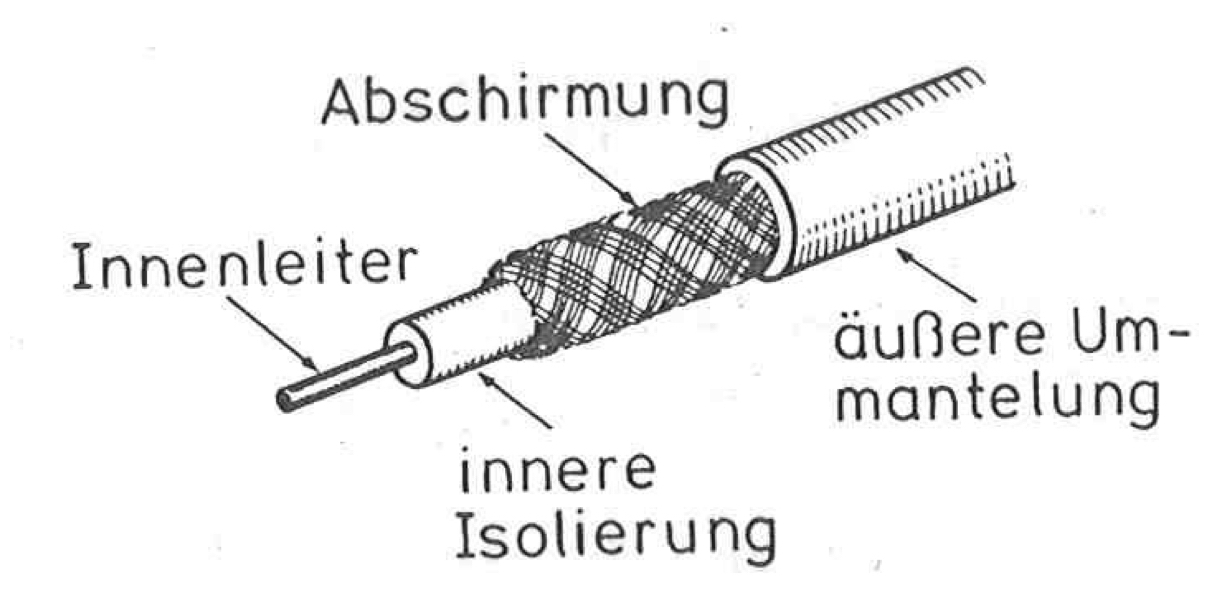
\includegraphics[width=\textwidth]{KoaxialKabel.jpeg}
    \caption{Aufbau eines Koaxialkabels und Schaltsymbol (unten rechts) \citep{VA}}
    \label{fig:Koaxialkabel}
\end{figure}

\newpage
\section{Erdschleifen}
Im vorherigen Abschnitt wurde bereits der Begriff Erdschleifen genannt, welcher nun genauer erklärt werden soll. Wenn die Abschirmungen verschiedener Apparaturen nicht miteinander verbunden sind, sondern jede einzeln geerdet ist, dann existieren dennoch kleine Potenzialunterschiede, die elektrostatisch in das System eingekoppelt werden und somit Störungen verursachen. Um Erdschleifen zu vermeiden, sollten alle Abschirmungen verbunden sein und an einem einzigen Erdungspunkt geerdet werden \citep{VA}. In Abbildung \ref{fig:Erdschleife} wird dies schematisch dargestellt.
\begin{figure}[h]
    \centering
    \begin{subfigure}{0.45\textwidth}
        \centering
        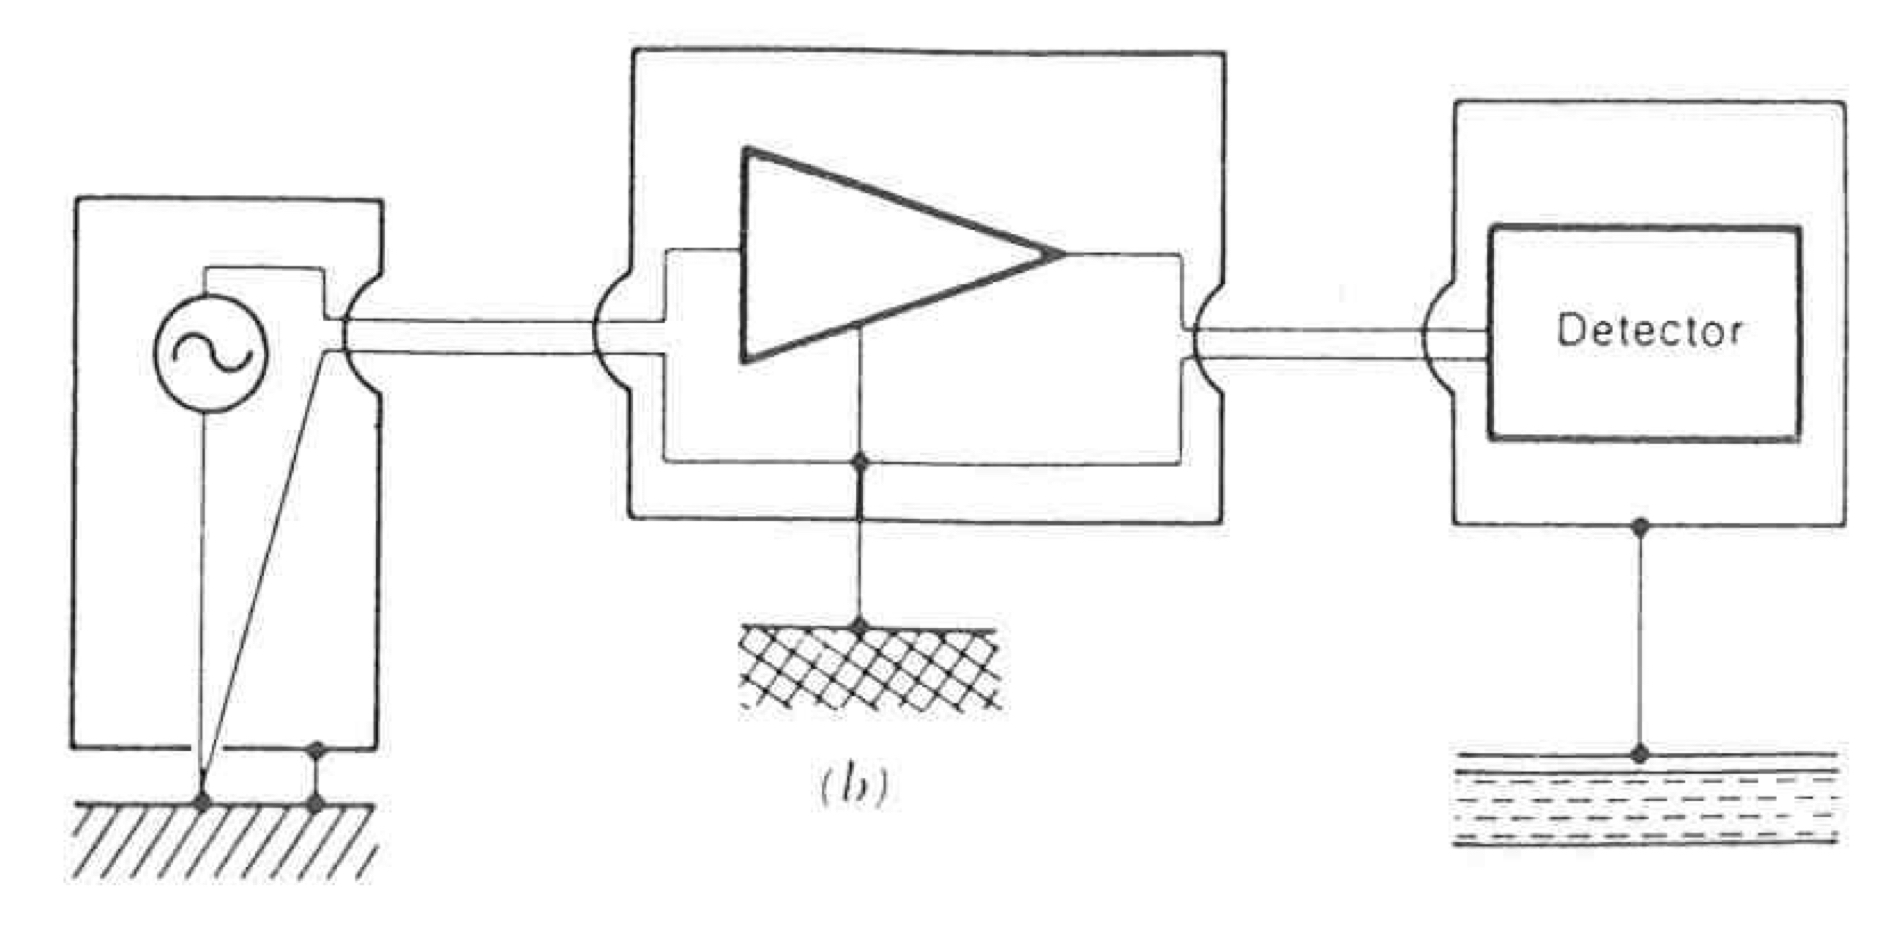
\includegraphics[width=\textwidth]{Erdschleife.jpeg}
        \caption{Falsche Erdung \citep{VA}}
    \end{subfigure}
    \hfill 
    \begin{subfigure}{0.45\textwidth}
        \centering
        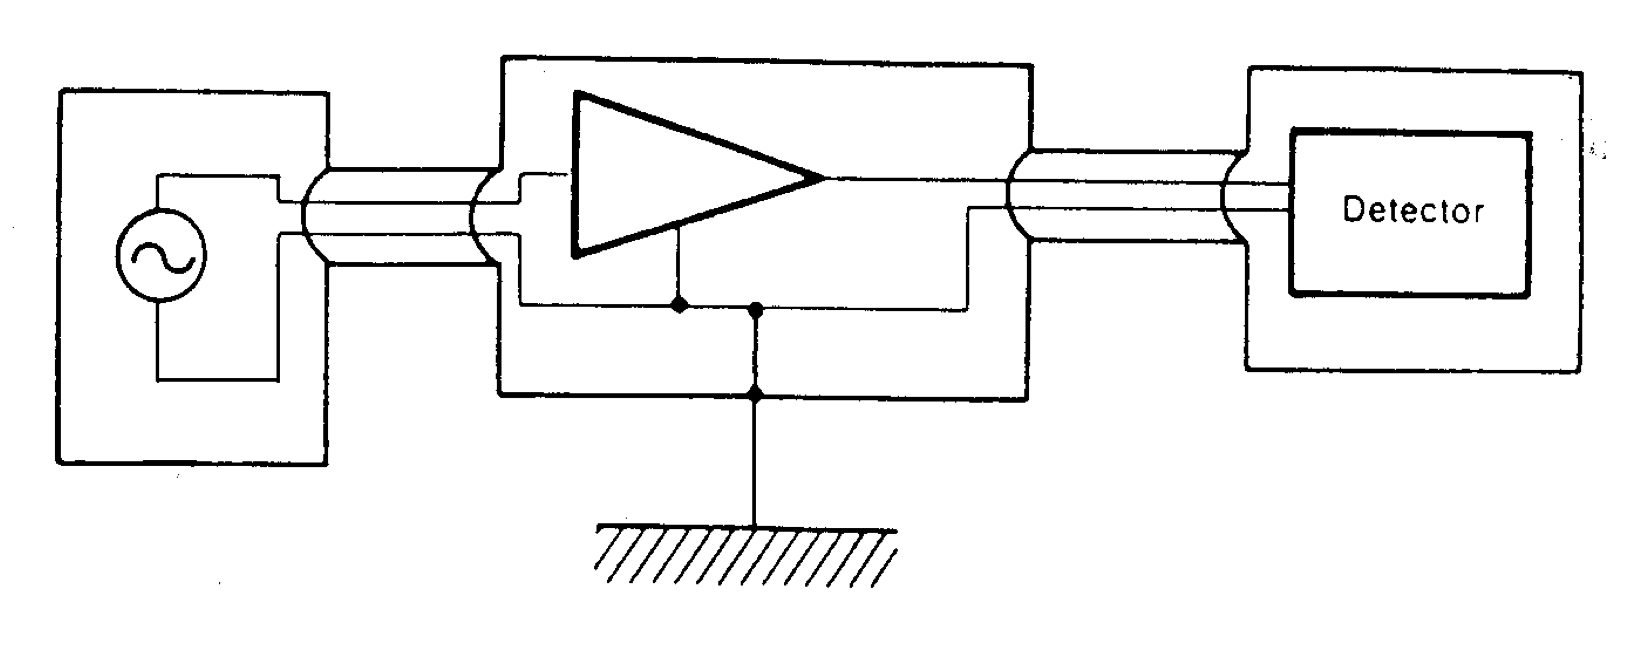
\includegraphics[width=\textwidth]{keineErdschleife.jpeg}
        \caption{Richtige Erdung \citep{VA}}
    \end{subfigure}
    \caption{Beispiele für falsche und richtige Erdung}
    \label{fig:Erdschleife}
\end{figure}